\documentclass[12pt]{article}
\usepackage{preamble}

\pagestyle{fancy}
\fancyhead[LO,LE]{Дополнительные главы \\ высшей математики}
\fancyhead[CO,CE]{15.11.2024}
\fancyhead[RO,RE]{Лекции Далевской О. П.}

\fancyfoot[L]{\scriptsize исходники найдутся тут: \\ \url{https://github.com/pelmesh619/itmo_conspects} \Cat}

\begin{document}
    \Mem Решаем задачу о перпендикуляре, ищем $f_0$ - наименьшую из проекций и минимально отстоящую от $f$

    Координаты $f_0$ в выбранном ортонормированном базисе $L^\prime$ равны соответствующим координатам $f$ в этом базисе

    $f_0 = \underset{k = \dim L^\prime, n = \dim L}{f_1 e_1 + f_2 e_2 + \dots + f_k e_k} = 
    (f, e_1) e_1 + (f, e_2) e_2 + \dots + (f, e_k) e_k$

    $(f, e_1) = \int_a^b f(x) e_1(x) dx$

    \Nota Итак, $\letsymbol L \in C_{[-\pi, \pi]}, L^\prime = l_{\{1, \sin x, \cos x, \sin 2x, \cos 2x, \dots\}}$

    Тогда можно искать многочлен $P_n(x) = \frac{a_0}{2} + a_1 \cos x + b_1 \sin x + \dots + a_n \cos nx + b_n \sin x$, который
    наилучшим образом приближает $f(x)$

    Если нормировать систему $\{\sin nx, \cos nx\}$, то коэффициентами многочлена $P_n(x)$ будут скалярные произведения
    $f(x)$ на функция ортонормированной системы. 
    
    Получим $\left\{\frac{1}{2\pi}, \frac{\sin x}{\pi}, \frac{\cos x}{\pi}, \dots, \frac{\sin nx}{\pi}, \frac{\cos nx}{\pi}\right\}$

    {
        \begin{tabular}{l|l|l}
            \cline{2-2}
            Тогда, & $\frac{a_0}{2} = \frac{1}{2\pi} \int_{-\pi}^\pi f(x) dx$ & \\
            & $a_k = \frac{1}{\pi} \int_{-\pi}^\pi f(x) \cos kx dx$ & - коэффициенты Фурье \\
            & $b_k = \frac{1}{\pi} \int_{-\pi}^\pi f(x) \sin kx dx$ & \\
            \cline{2-2}
        \end{tabular}
    }

    \Nota Если увеличивать степень $n$, то получим ряд Фурье. Запишем формально:

    $\frac{a_0}{2} + \sum_{n = 1}^\infty (a_n \cos nx + b_n \sin nx)$ - сходится ли этот ряд и сходится ли к $f(x)$?

    Ответ дает теорема (доказательство будет приведено позже)

    \begin{MyTheorem}
        \Ths $f(x)$ - $2\pi$-периодична, на $[-\pi, \pi]$ $f(x)$ - кусочно монотонна и ограничена (то есть имеет конечное число конечных разрывов). 
        Тогда в точках непрерывности $f(x)$ представляется рядом Фурье:
        
        \[f(x) = \frac{a_0}{2} + \sum_{n = 1}^\infty (a_n \cos nx + b_n \sin nx) = S(x)\]

        а в точках разрыва $S(x_0) = \frac{1}{2} (f(x_0 + 0) + f(x_0 - 0))$
    \end{MyTheorem}

    Сейчас только тригонометрический ряд Фурье, хотя подобное разложение возможно 
    по различным ортогональным системам функций

    \Nota В концах отрезках $[-\pi, \pi]$ $f(x)$ может быть не определена, но в любом случае ограничена $S(\pi) = S(-\pi) = \frac{1}{2} (f(-\pi + 0) + f(\pi - 0))$

    \mediumvspace

    \underline{Разложение периодичных функций} (на $[-\pi, \pi]$)

    1$^\circ$: $f(x) = x$ на $[-\pi, \pi]$, $f(x + 2\pi) = f(x)$

    $\frac{a_0}{2} = \frac{1}{2\pi} \int_{-\pi}^\pi x dx = 0$

    $a_n = \frac{1}{\pi} \int_{-\pi}^\pi x \cos nx dx = 0$

    $b_n = \frac{1}{\pi} \int_{-\pi}^\pi x \sin nx dx = \frac{-2}{\pi n} \int_{0}^\pi xd\cos nx = -\frac{2}{\pi n} \left(x \cos nx \Big|_0^\pi - \cancelto{0}{\int_0^\pi \cos nx dx}\right) = 
    -\frac{2}{\pi n} x \cos nx \Big|_0^\pi = -\frac{2}{n} \cos \pi n = \begin{sqcases}\frac{-2}{n}, & n = 2m \\ \frac{2}{n}, & n = 2m + 1\end{sqcases} = \frac{2}{n} (-1)^{n + 1}$

    Итак $f(x) = \sum_{n = 1}^\infty \frac{(-1)^{n + 1} \cdot 2}{n} \sin nx$

    \begin{center}
        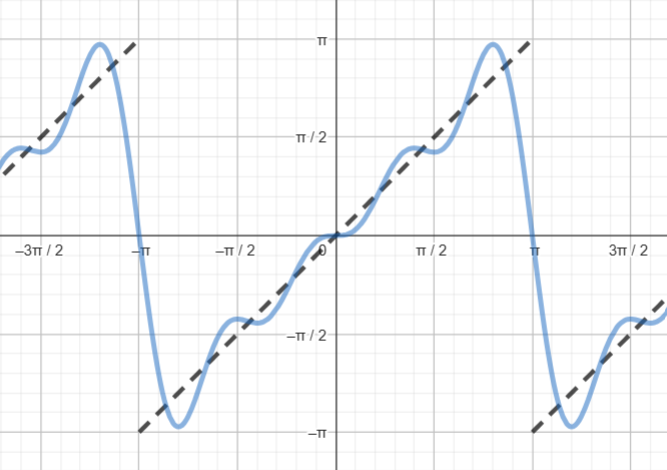
\includegraphics[width=0.5\textwidth]{addchapters1/images/addchapters1_2024_11_15_1}
    \end{center}

    2$^\circ$: $f(x) = \begin{cases}1 & \text{на } [0, \pi] \\ -1 & \text{на } [-\pi, 0)\end{cases}$ на $[-\pi, \pi]$

    $\frac{a_0}{2} = \frac{1}{2\pi} \int_{-\pi}^\pi f(x) dx = 0$

    $a_n = \frac{1}{\pi} \int_{-\pi}^\pi f(x) \cos nx dx = 0$

    $b_n = \frac{1}{\pi} \int_{-\pi}^\pi f(x) \sin nx dx = \frac{1}{\pi} \left(-\int_{-\pi}^0 \sin nx dx + \int_0^\pi \sin nx dx\right) = 
    \frac{1}{2n} \left(\int_{-\pi}^0 d\cos nx - \int_0^\pi d\cos nx\right) = \frac{1}{\pi n} \left(\cos nx \Big|_{-\pi}^0 - \cos nx \Big|_0^\pi\right) = 
    \frac{1}{\pi n} (1 - \cos \pi n - \cos \pi n + 1) = \frac{2}{\pi n}(1 - \cos \pi n) = \frac{4}{\pi (2m - 1)}$

    $f(x) = \sum_{m = 1}^\infty \frac{4}{\pi (2m - 1)} \sin (2m - 1) x$

    \begin{center}
        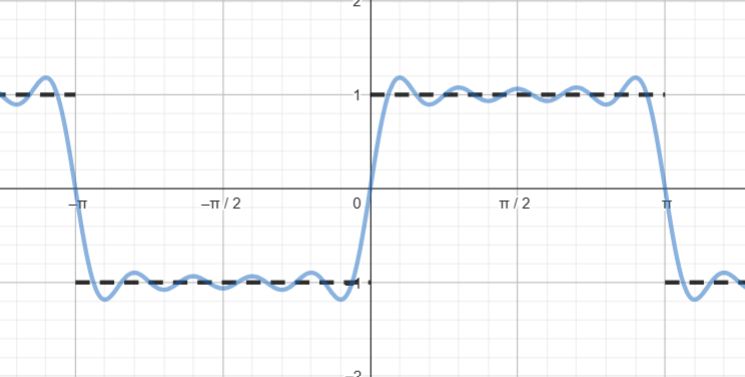
\includegraphics[width=0.5\textwidth]{addchapters1/images/addchapters1_2024_11_15_2}
    \end{center}

    \Nota Заметим, что если $f(x)$ - четная, то $b_n = 0$, а если нечетная, то $a_n = 0$. Иногда в задаче
    требуется разложить $f(x)$, заданную только на отрезке $[0, \pi]$. Такую функцию можно продолжить четным
    или нечетным образом на $[-\pi, \pi]$. Говорят о разложении в ряд по косинусам и синусам соответственно

    3$^\circ$: $f(x) = \pi - x, \quad x \in [0, \pi]$

    Дополним $f(x)$ двумя способами

    \begin{multicols}{2}
        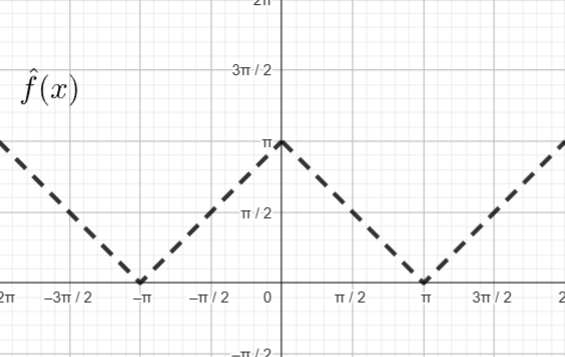
\includegraphics[width=0.5\textwidth]{addchapters1/images/addchapters1_2024_11_15_4}

        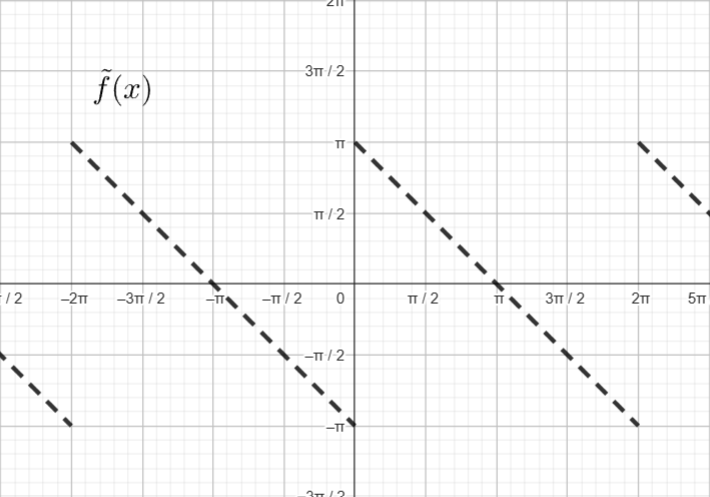
\includegraphics[width=0.5\textwidth]{addchapters1/images/addchapters1_2024_11_15_3}
    \end{multicols}

    В ряд Фурье раскладывются периодические функции $\hat{f}, \tilde{f}$

    \Lab $\hat{f}(x) = \frac{a_0}{2} + \sum_{n = 1}^\infty a_n \cos nx \quad\quad\quad \tilde{f}(x) = \sum_{n = 1}^\infty b_n \sin nx$

    \mediumvspace

    \begin{multicols}{2}
        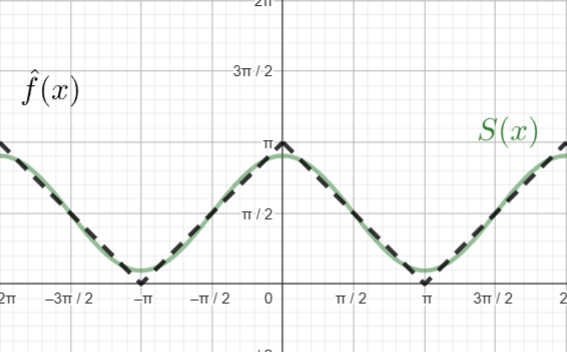
\includegraphics[width=0.5\textwidth]{addchapters1/images/addchapters1_2024_11_15_5}

        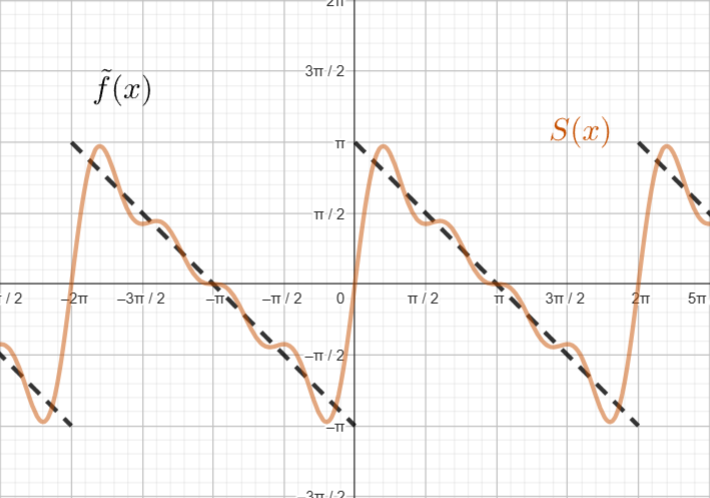
\includegraphics[width=0.5\textwidth]{addchapters1/images/addchapters1_2024_11_15_6}
    \end{multicols}

    \mediumvspace

    Заметим, что $\tilde{f}$ на $[0, 2\pi]$ имеет одно аналитическое задание (удобно интегрировать). Изменится ли 
    ряд Фурье, если сдвинуть отрезок?

    \begin{MyTheorem}
        \ThNs{о сдвиге} Сдвиг промежутка длиной $2\pi$ не меняет ряда Фурье
    \end{MyTheorem}

    \begin{MyTheorem}
        \ThNs{о растяжении} Для $f : [a, b] \to \Real$ растяжение промежутка приводит к разложению:

        $b - a = 2l = T$ - период

        $a_0 = \frac{1}{l} \int_{-l}^l f(x) dx$

        $a_n = \frac{1}{l} \int_{-l}^l f(x) \cos \frac{\pi n}{l} x dx$

        $b_n = \frac{1}{l} \int_{-l}^l f(x) \sin \frac{\pi n}{l} x dx$
    \end{MyTheorem}


\end{document}
